\subsection{Results}


\subsubsection{Total cross section and \texorpdfstring{$\BRgamgam/\BRZZ$}{BRgg/BRZZ}}

\tk{TODO: This is literal text from the paper}

The total cross section for Higgs boson production is measured to be
$61.1   \pm 6.0 \,\text{(stat)}   \pm 3.7 \,\text{(syst)}  $\pb
, based on a combination of the $\hgg$ and $\hzz$ channels, using the treatment described in Section 4 to the inclusive cross section (i.e. with a single bin, both at generator and at reconstruction level).
% 
The measured total cross sections from the individual channels are $64.0\pm9.6$\pb for $\hgg$ and $58.2\pm9.8$\pb for $\hzz$.
% 
The likelihood scans for the individual decay channels and their combination are shown in Fig.~\ref{fig:RatioOfbrsAndTotalXSscan}~(left).
% 
The combination result agrees with the current SM value of $55.6\pm2.5$\pb~\cite{deFlorian:2016spz}.


A measurement of the branching fraction for one decay channel is degenerate with a measurement of the total cross section.
% 
However, the ratio of branching fractions for two decay channels can be measured while profiling the total cross section.
% 
The ratio of the $\hgg$ and $\hzz$ branching fractions, $\BRgamgam/\BRZZ$, is measured to be
$0.092   \pm 0.018 \,\text{(stat)}   \pm 0.010 \,\text{(syst)}  $.
% 
This is in agreement with the SM prediction of $0.086 \pm 0.002$~\cite{deFlorian:2016spz}.
% 
The likelihood scan for $\BRgamgam/\BRZZ$ is shown in Fig.~\ref{fig:RatioOfbrsAndTotalXSscan}~(right).


\begin{figure}[hbtp]
  \begin{center}
    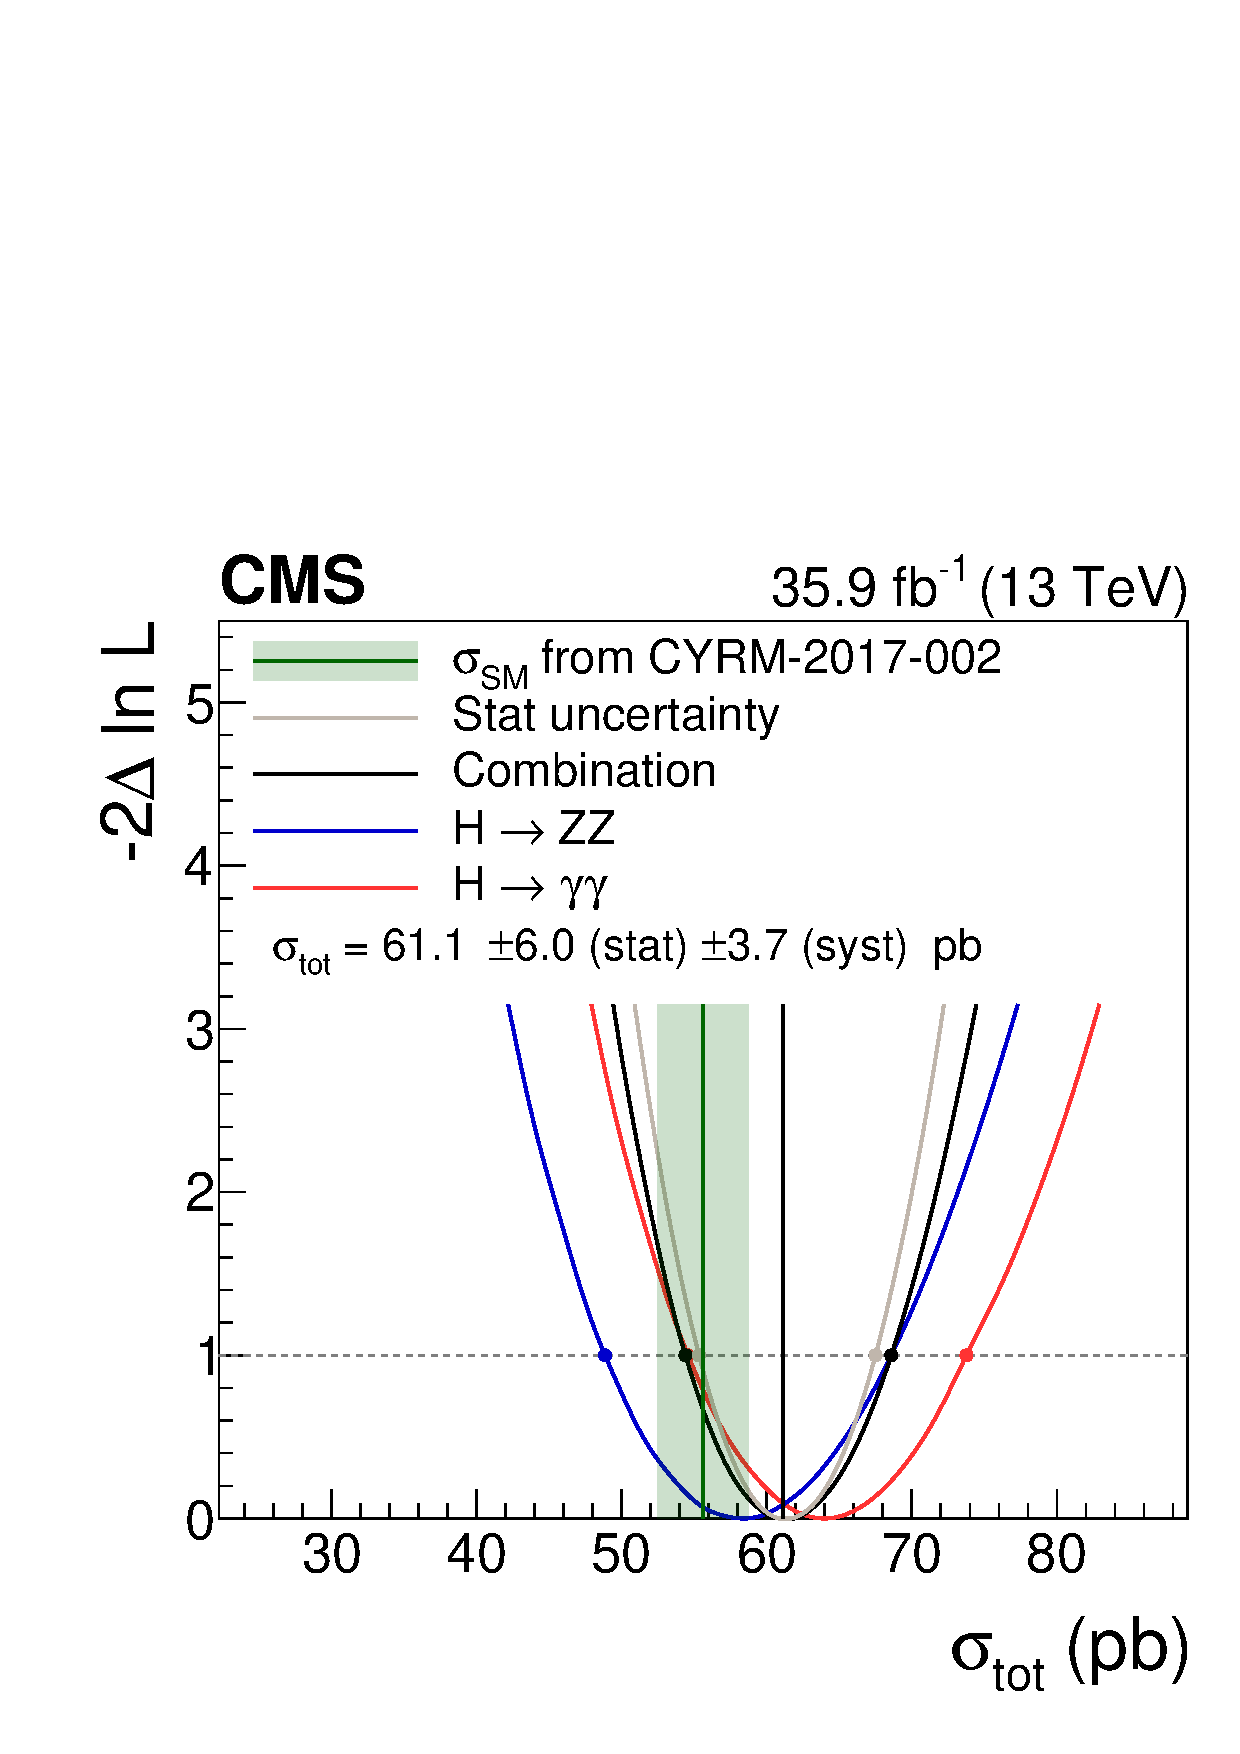
\includegraphics[width=0.49\linewidth]{img/differentials/scans_totalXS.pdf}
    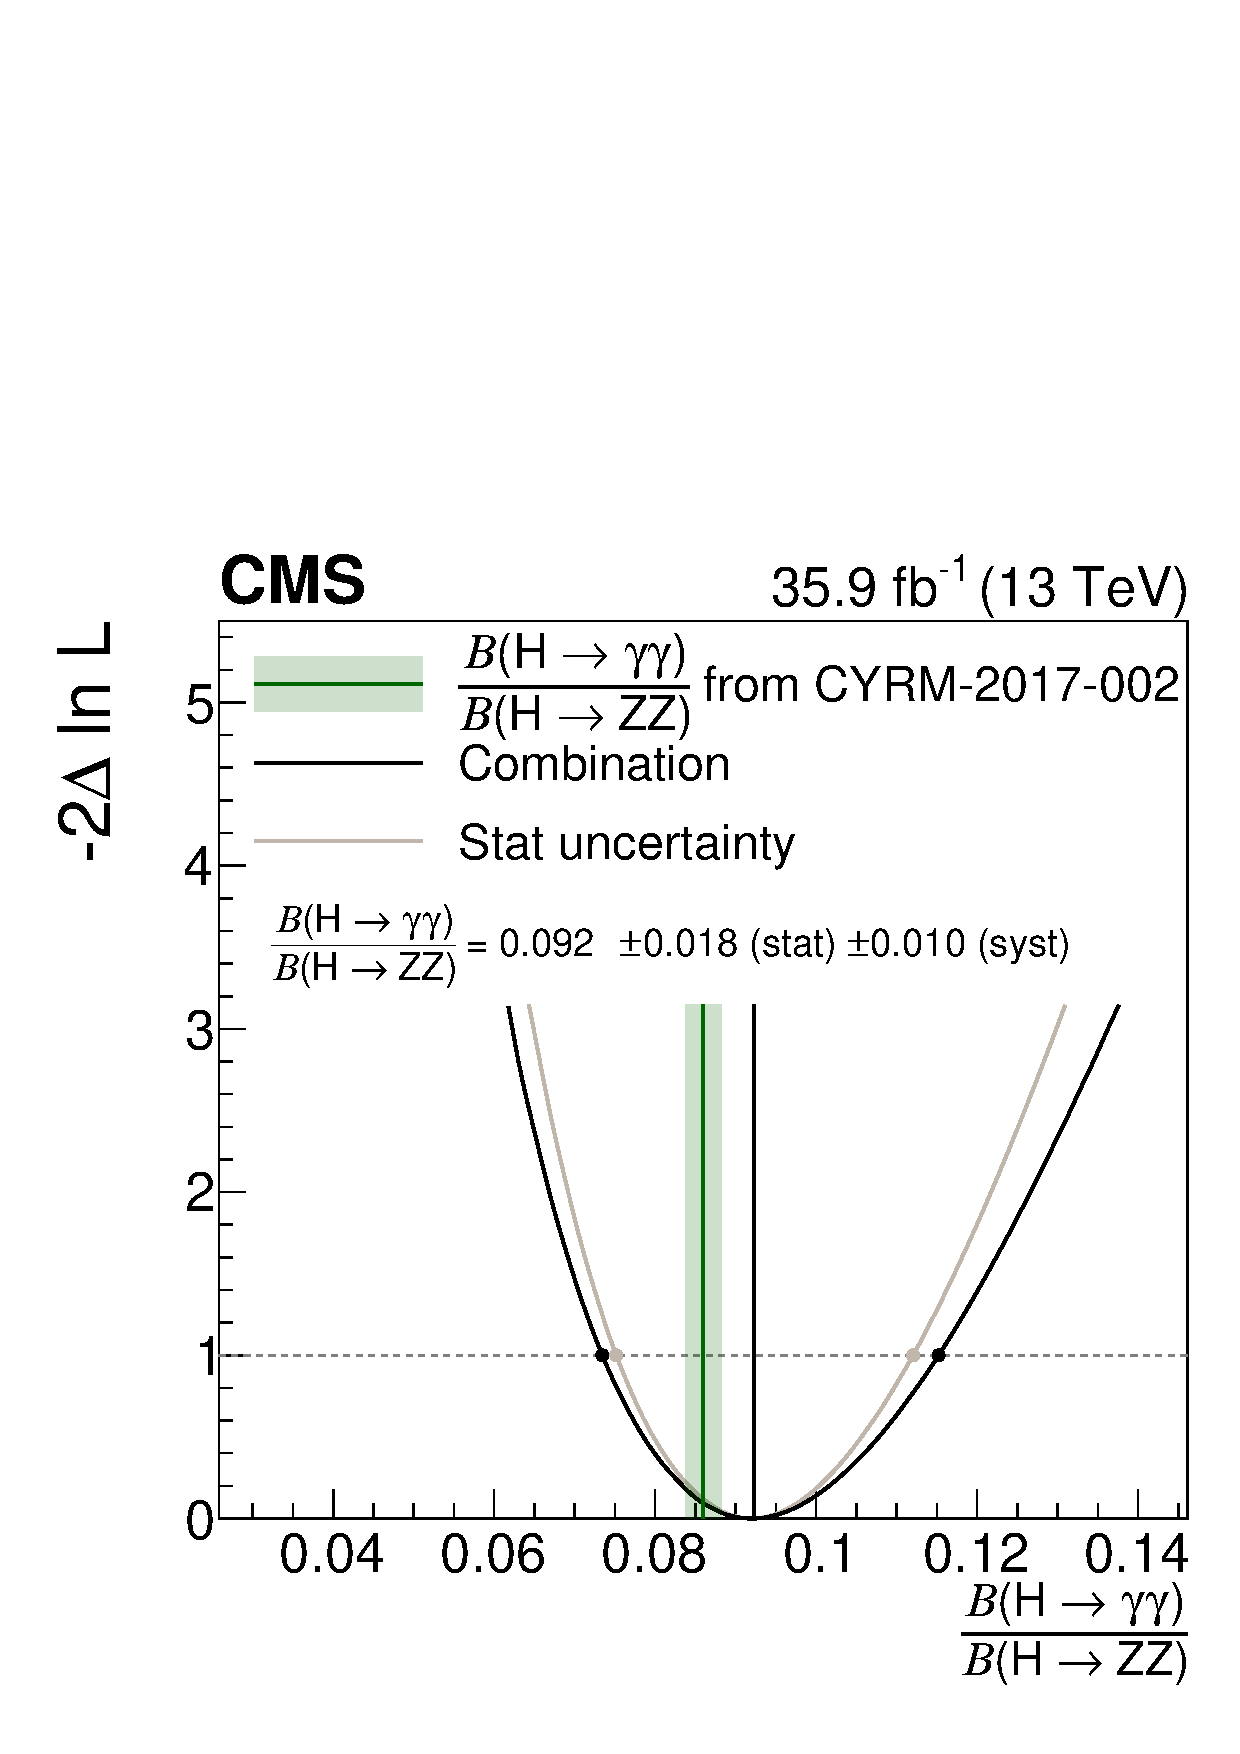
\includegraphics[width=0.49\linewidth]{img/differentials/scans_ratioOfBRs.pdf}
    \caption{
        Scan of the total cross section $\sigma_\text{tot}$ (left) and of the ratio of branching fractions $\BRgamgam/\BRZZ$ (right), based on a combination of the $\hgg$ and $\hzz$ analyses.
        % 
        The measured total cross sections from the individual channels are $64.0\pm9.6$\pb for $\hgg$ and $58.2\pm9.8$\pb for $\hzz$.
        % 
        The markers indicate the one standard deviation confidence interval.
        }
    \label{fig:RatioOfbrsAndTotalXSscan}
  \end{center}
\end{figure}



\subsubsection{Combinations of differential observables}

\tk{TODO: This is literal text from the paper}

The unfolded differential cross sections for the observables $\pth$, $\njets$, $\absy$, and $\ptjet$ are shown in
Figs.~\ref{fig:CombinedSpectra_pth}, \ref{fig:CombinedSpectra_njets}, \ref{fig:CombinedSpectra_rapidity}, and \ref{fig:CombinedSpectra_ptjet}, respectively.
% 
Figure~\ref{fig:CombinedSpectra_pth} (right) shows the differential cross section of $\pth$ for Higgs boson production via gluon fusion;
% 
for this result, the non-gluon-fusion production modes are considered to be background, constrained to the SM predictions with their respective uncertainties.
% 
% an uncertainty on the inclusive cross section of non-gluon-fusion production modes is taken into account~\cite{deFlorian:2016spz}.
% 
% For the other differential cross sections, no distinction is made regarding the production mode.
% 
% including differential cross sections for Higgs boson production via gluon fusion for the observable $\pth$.
% 
Corresponding bin-to-bin correlation matrices are given in Appendix~\ref{sec:binToBinCorrelationMatrices}.
% 
For the observables $\pth$, $\njets$, and $\ptjet$, the rightmost bin is an overflow bin, which is normalized by the bin width of the second-to-rightmost bin.
% 
% Here the cross section is divided by the bin width of the second-to-rightmost bin, giving these two bins the same normalization (\ie, if the integrated cross sections in the rightmost and second-to-rightmost bin were equal, their displayed values on the $y$ axis would be the same).
% 
% (ensuring that if the integrated cross sections in the last and second-to-rightmost bin are equal, the value in the histogram is the same).
% 
Overall no significant deviations from the SM predictions are observed.
% 
For the $\pth$ spectrum, the dominant source of uncertainty is the statistical one; in particular, the systematic uncertainty is about half the statistical uncertainty in the rightmost bin, and much smaller than the statistical uncertainty in all other bins.
% 
% For the $\pth$ spectrum, the uncertainties are statistically dominated; in particular, the systematic uncertainty is about half the statistical uncertainty in the rightmost bin, and much smaller in all other bins.
% 
The total uncertainty in the combination per bin varies between 30 and 40\%.
% 
Compared to the measurement in the $\hgg$ channel alone,
% Relative to the spectrum of the $\hgg$ analysis alone,
the decrease in uncertainty achieved by the combination is most notable in the low-$\pt$ region.
% 
% The overall uncertainties vary between 30\% and 40\%, and decrease with respect to the individual decay channels most notably in the lower $\pt$ region.
% % 
% Overall, the uncertainty of the combination with respect to only $\hgg$ is about 15\% smaller.
% 
The contribution of the $\hbb$ channel to the overall precision of the combination is most significant in the last $\pth$ bin.

\begin{figure}[hbtp]
  \begin{center}
    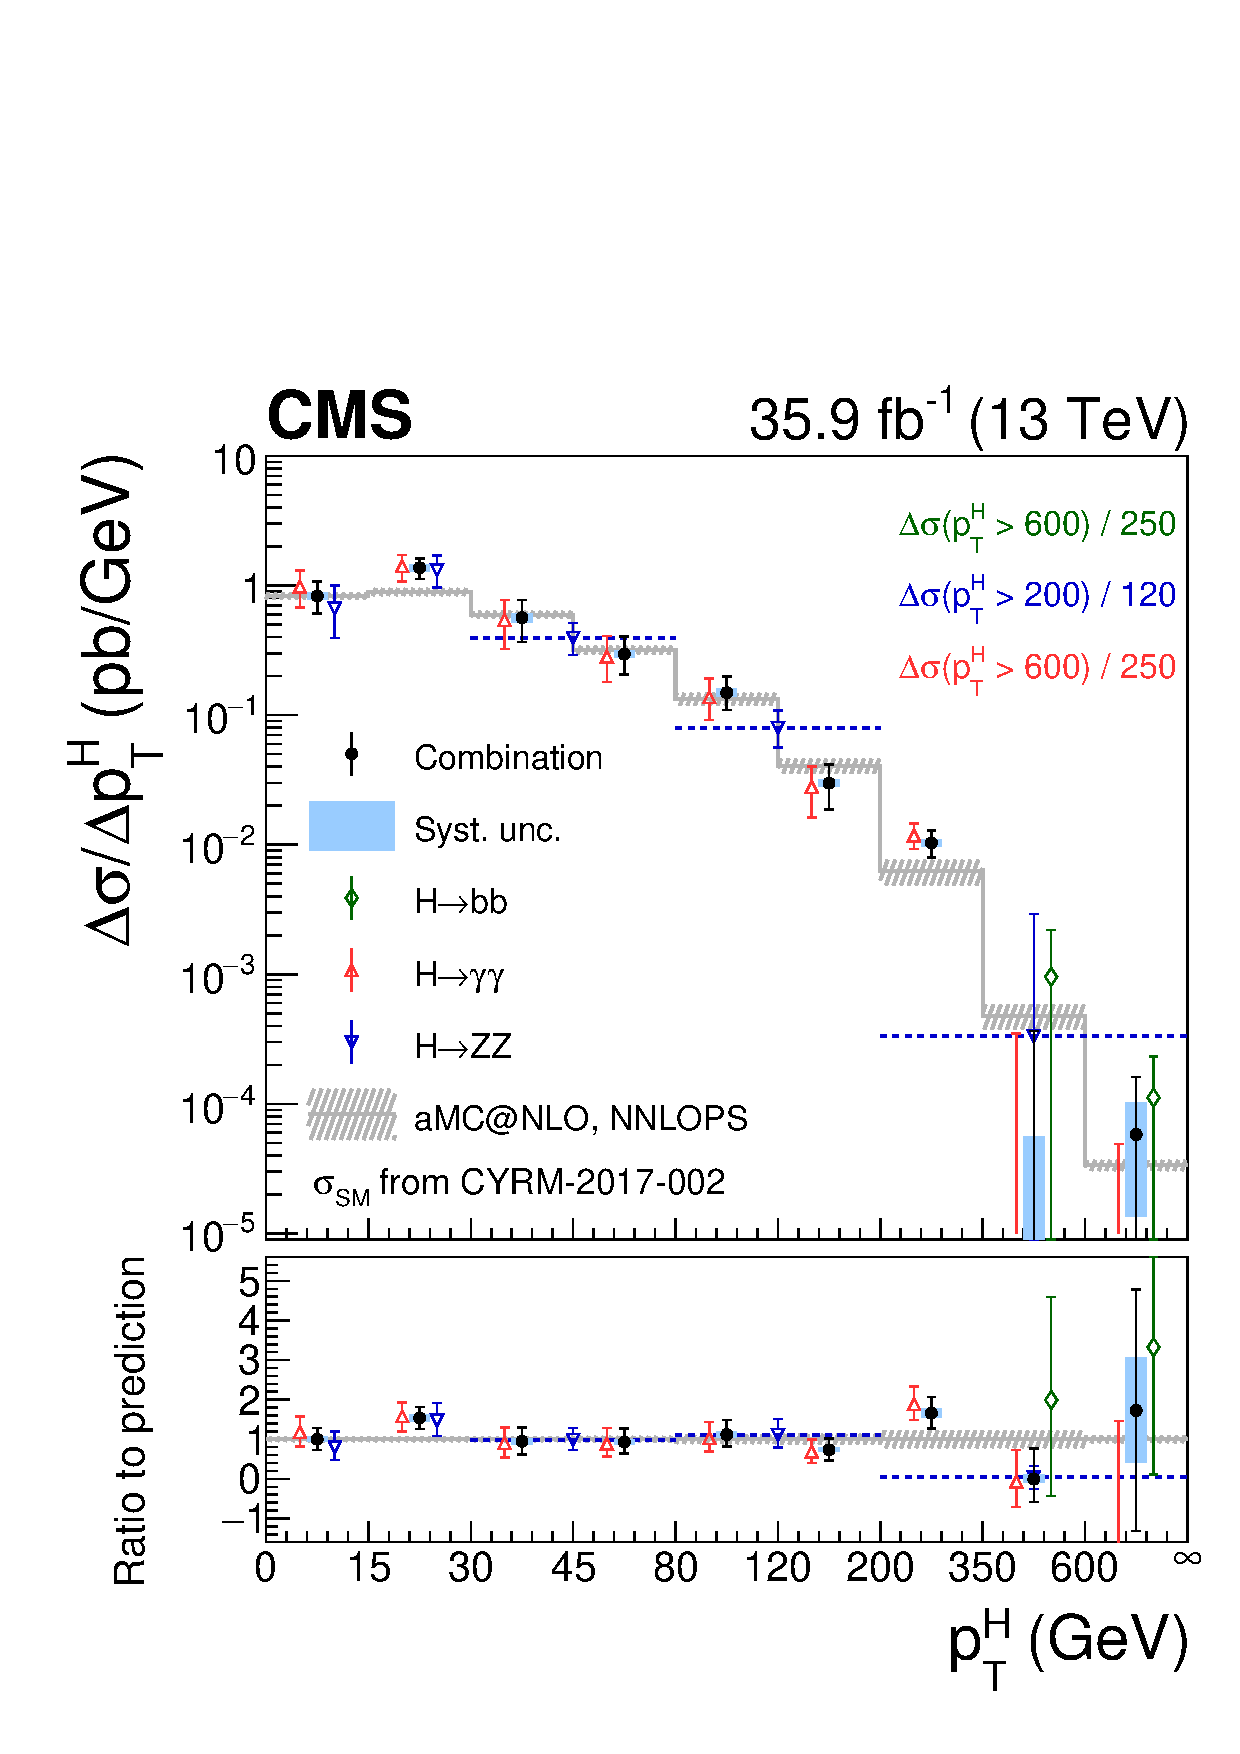
\includegraphics[width=0.49\linewidth]{img/differentials/spectra_pth_smH.pdf}
    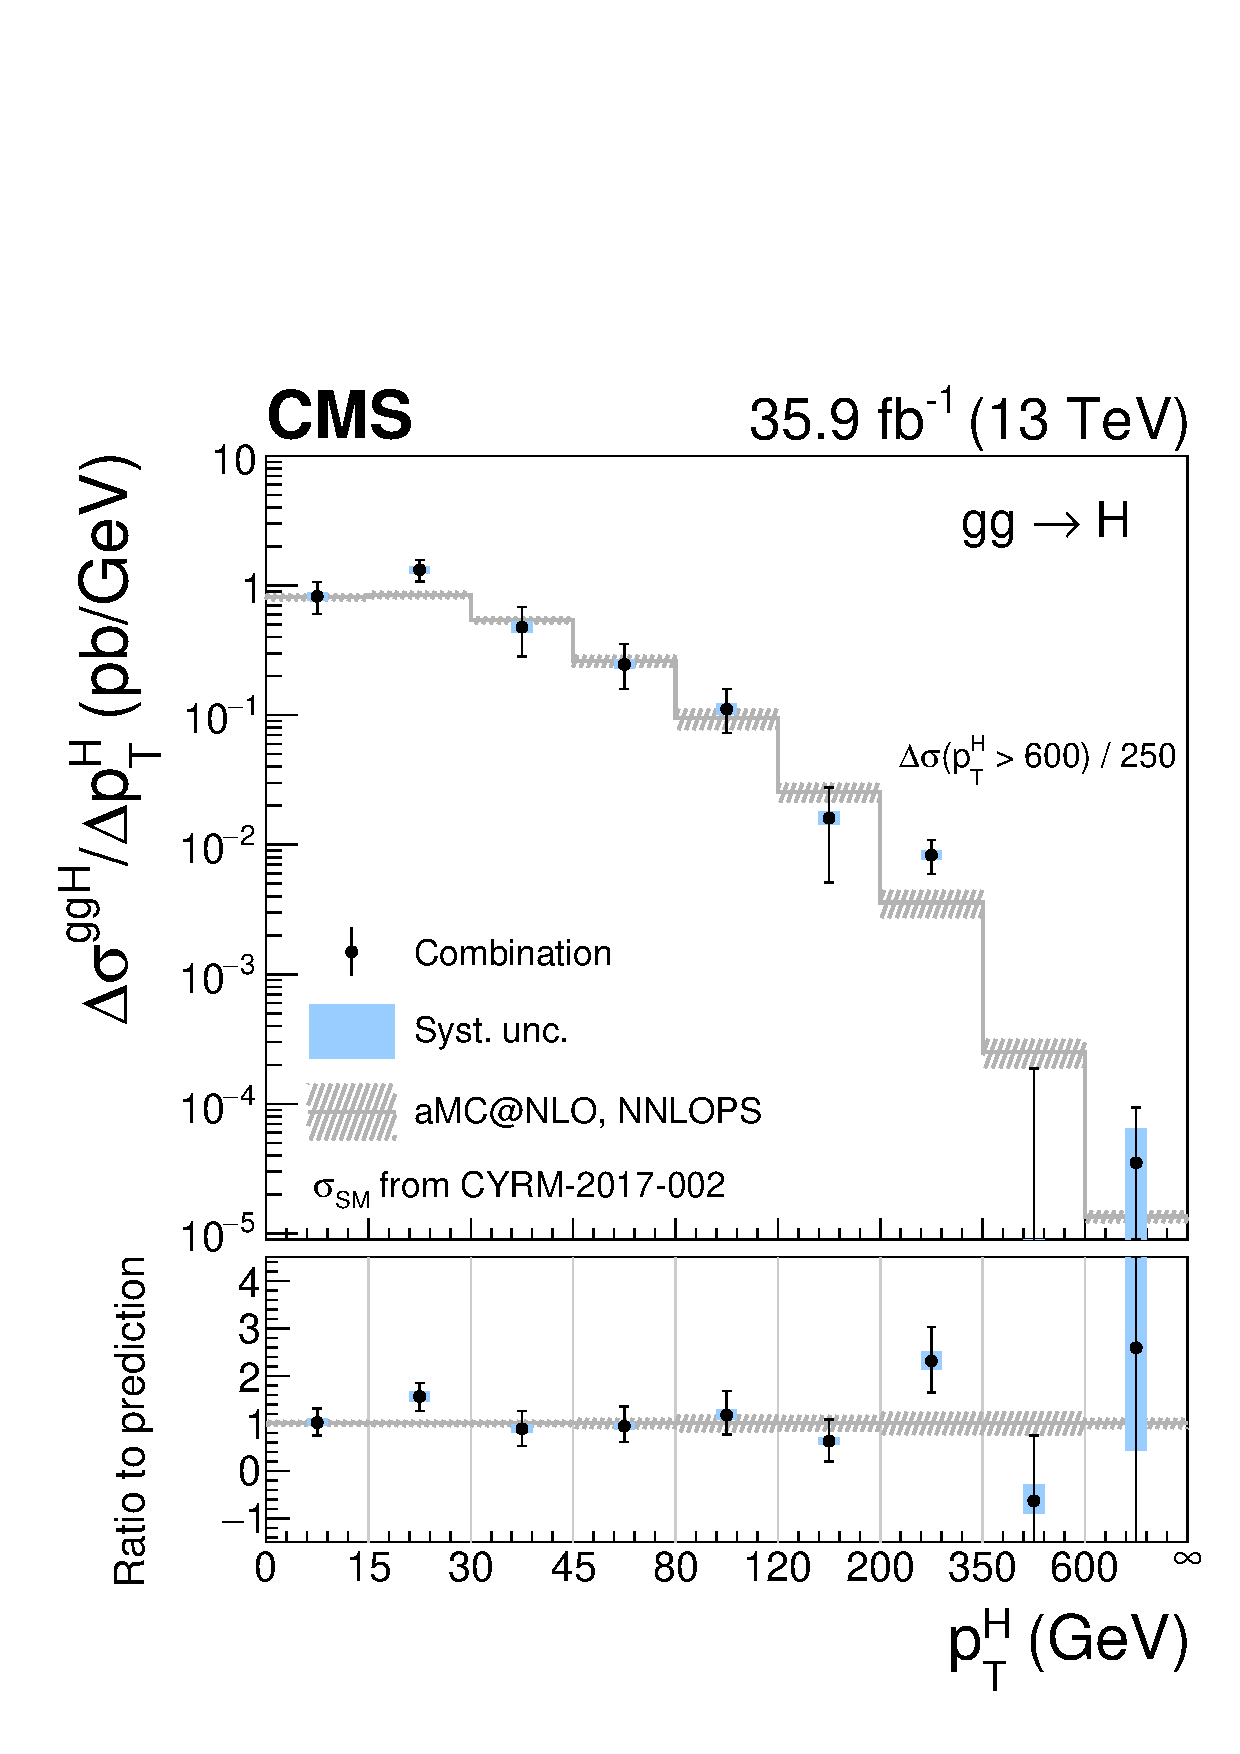
\includegraphics[width=0.49\linewidth]{img/differentials/spectra_pth_ggH.pdf}
    \caption{
        Measurement of the total differential cross section (left) and the differential cross section of gluon fusion (right) as a function of $\pth$. The combined spectrum is shown as black points with error bars indicating a 1 standard deviation uncertainty. The systematic component of the uncertainty is shown by a blue band. The spectra for the $\hgg$, $\hzz$, and $\hbb$ channels are shown in red, blue, and green respectively.
        % 
        The dotted horizontal lines in the $\hzz$ channel indicate that the measurement was carried out with a coarser binning.
        % 
        The rightmost bins of the distributions are overflow bins; the normalizations of the cross sections in these bins are indicated in the figure.
        }
    \label{fig:CombinedSpectra_pth}
  \end{center}
\end{figure}

\begin{figure}[hbtp]
  \begin{center}
    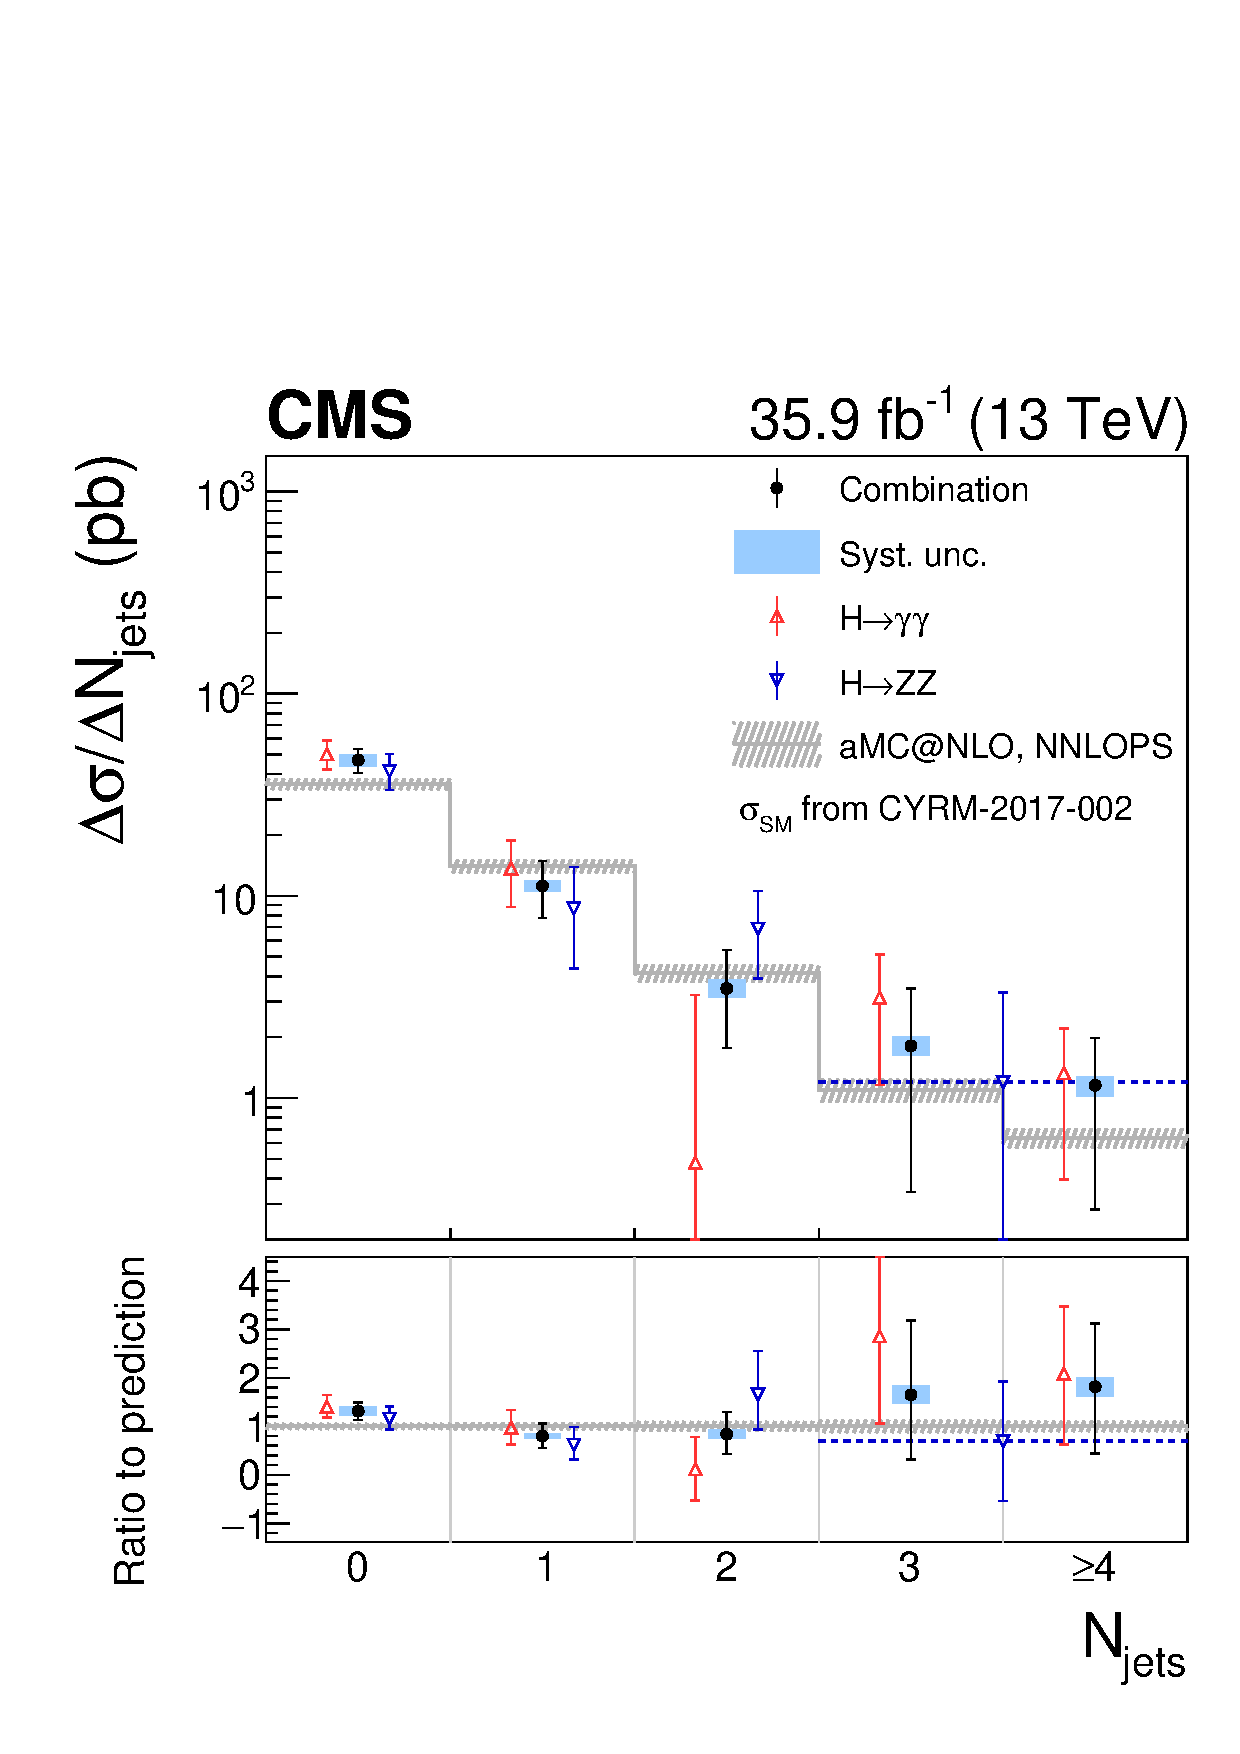
\includegraphics[width=0.49\linewidth]{img/differentials/spectra_njets.pdf}
    \caption{
        Measurement of the differential cross section as a function of $\njets$. The combined spectrum is shown as black points with error bars indicating a 1 standard deviation uncertainty. The systematic component of the uncertainty is shown by a blue band. The spectra for the $\hgg$ and $\hzz$ channels are shown in red and blue respectively.
        % 
        The dotted horizontal lines in the $\hzz$ channel indicate that the measurement was carried out with a coarser binning.
        }
    \label{fig:CombinedSpectra_njets}
  \end{center}
\end{figure}

\begin{figure}[hbtp]
  \begin{center}
    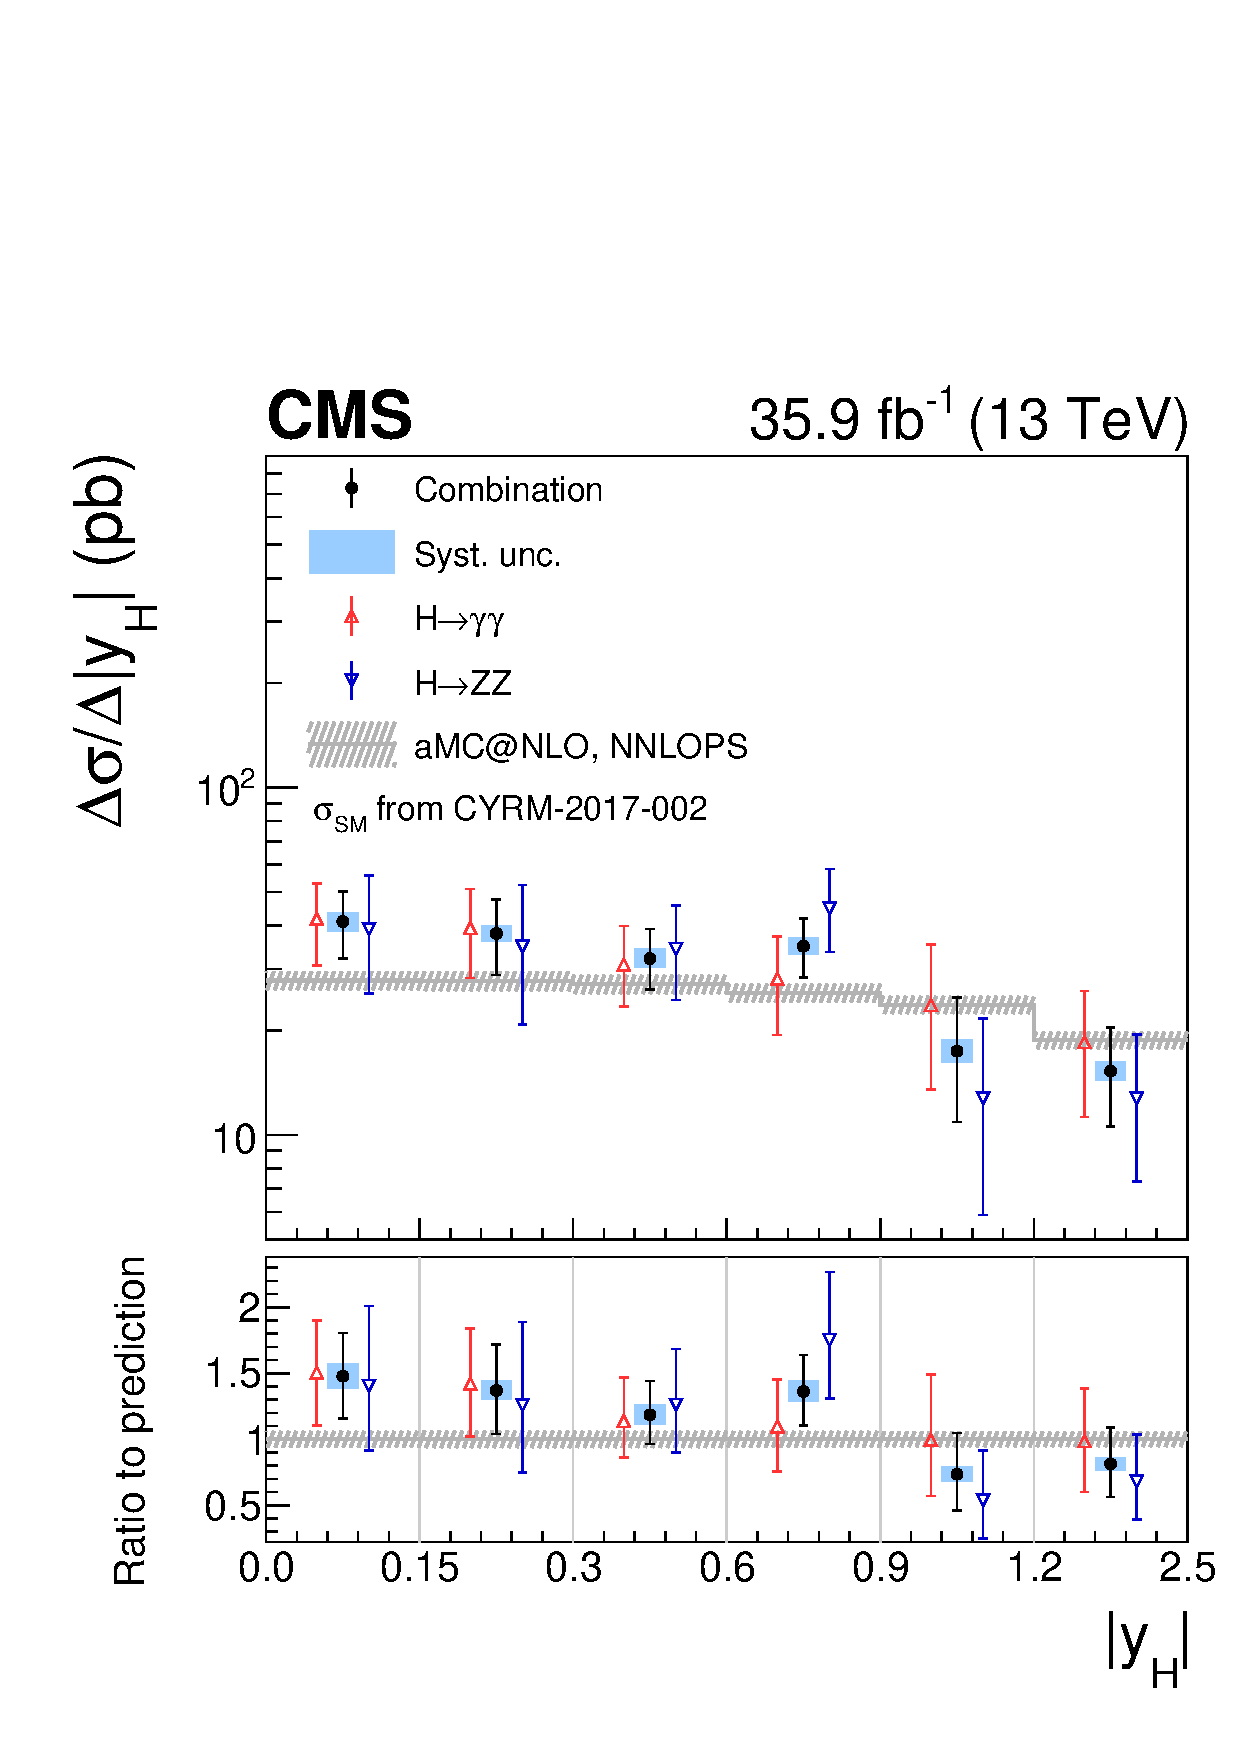
\includegraphics[width=0.49\linewidth]{img/differentials/spectra_rapidity.pdf}
    \caption{
        Measurement of the differential cross section as a function of $\absy$. The combined spectrum is shown as black points with error bars indicating a 1 standard deviation uncertainty. The systematic component of the uncertainty is shown by a blue band. The spectra for the $\hgg$ and $\hzz$ channels are shown in red and blue respectively.
        }
    \label{fig:CombinedSpectra_rapidity}
  \end{center}
\end{figure}

\begin{figure}[hbtp]
  \begin{center}
    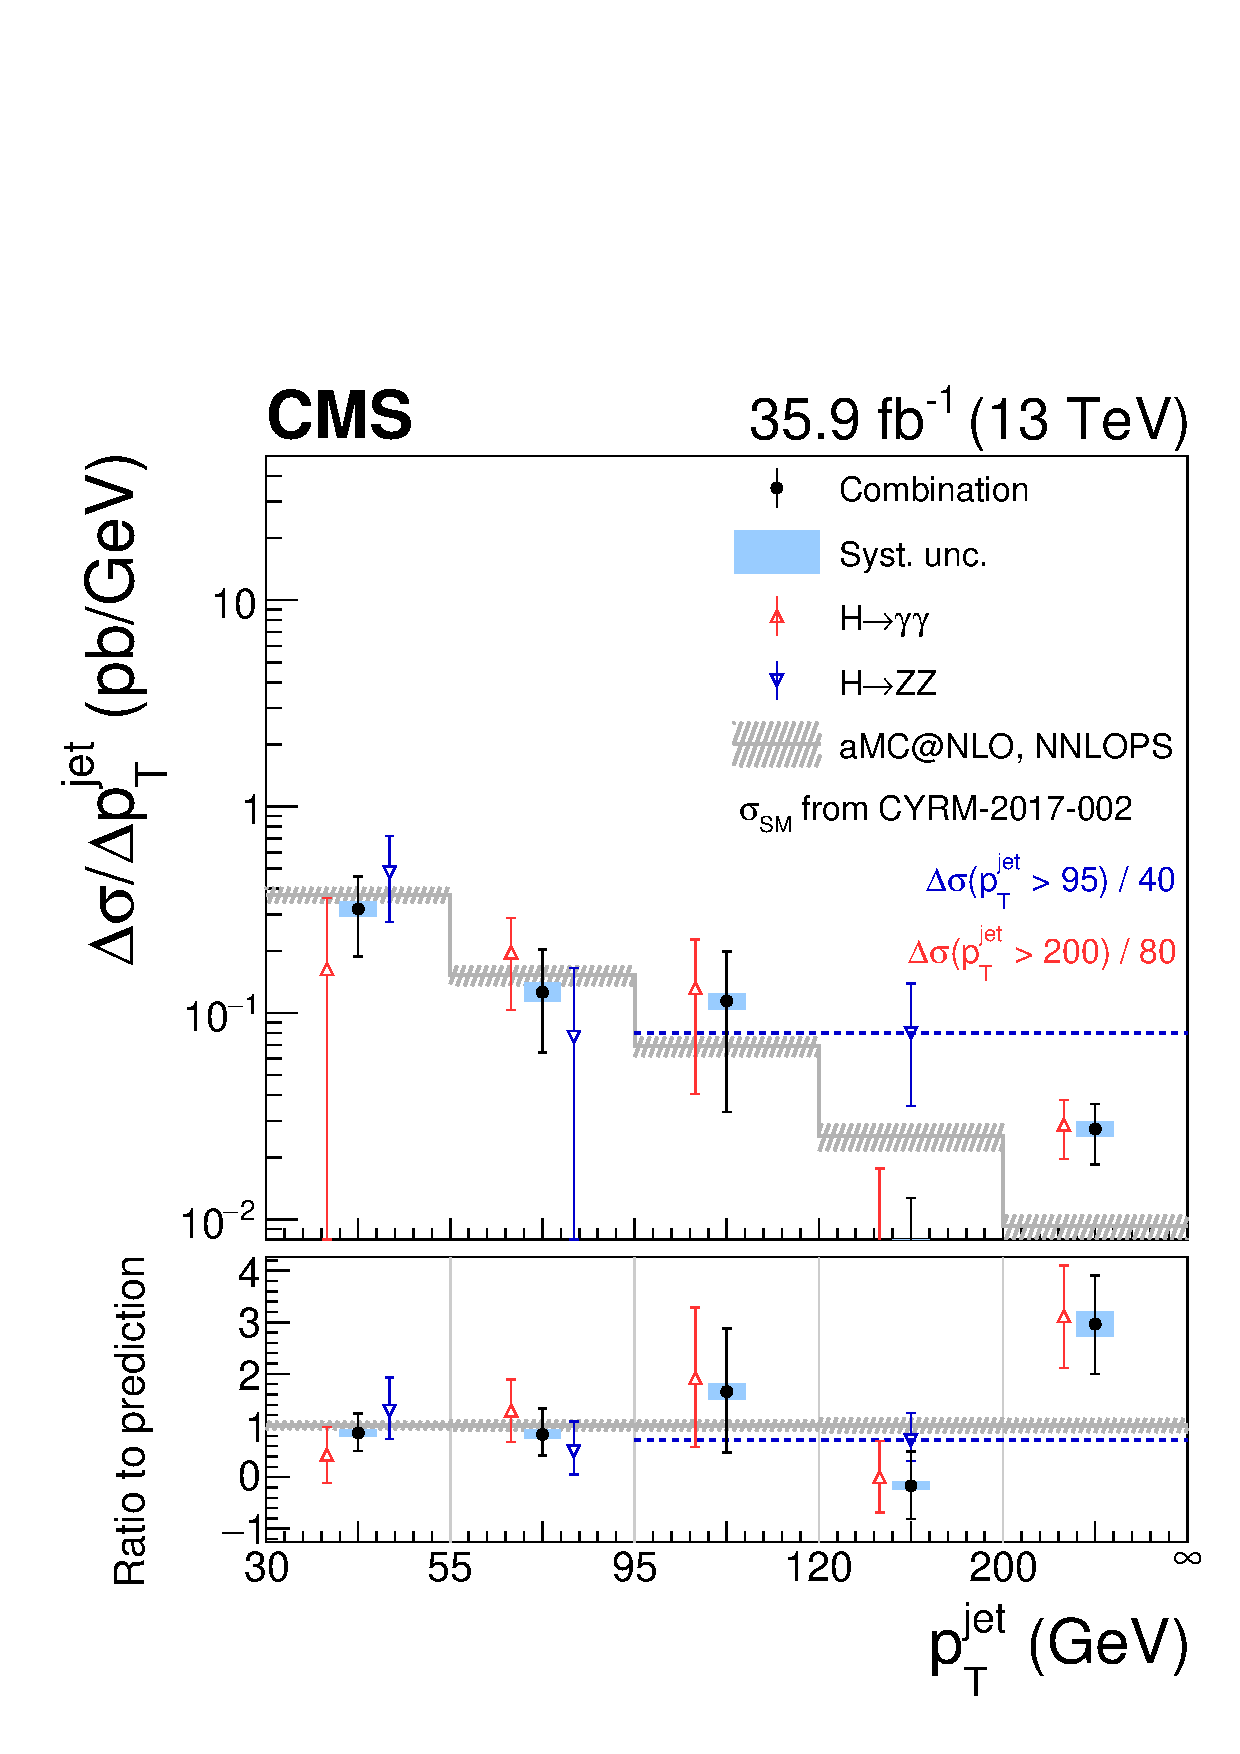
\includegraphics[width=0.49\linewidth]{img/differentials/spectra_ptjet.pdf}
    \caption{
        Measurement of the differential cross section as a function of $\ptjet$. The combined spectrum is shown as black points with error bars indicating a 1 standard deviation uncertainty. The systematic component of the uncertainty is shown by a blue band. The spectra for the $\hgg$ and $\hzz$ channels are shown in red and blue respectively.
        % 
        The dotted horizontal lines in the $\hzz$ channel indicate that the measurement was carried out with a coarser binning.
        % 
        The rightmost bin of the distribution is an overflow bin; the normalization of the cross section in that bin is indicated in the figure.
        }
    \label{fig:CombinedSpectra_ptjet}
  \end{center}
\end{figure}
